\documentclass[border=10pt]{standalone}
\usepackage{pgfplots}
\pgfplotsset{compat=1.18}
\begin{document}
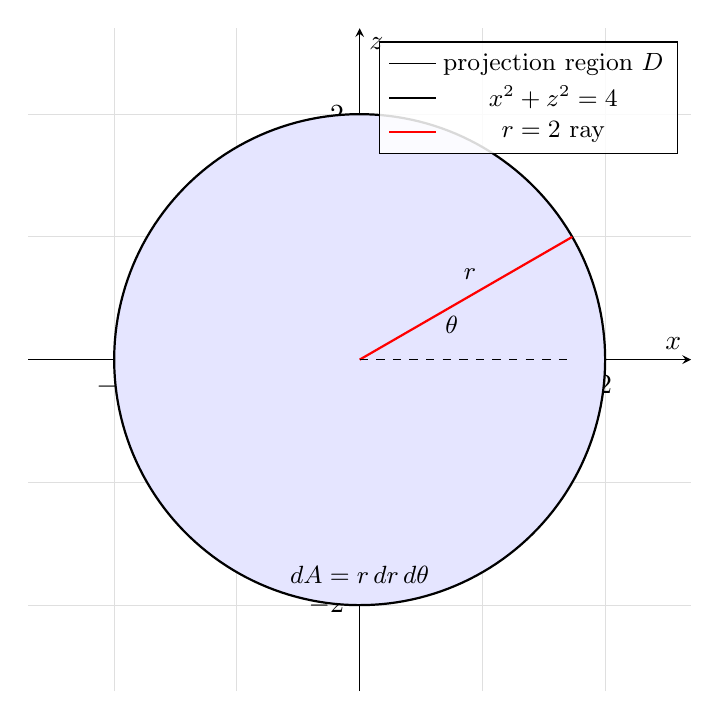
\begin{tikzpicture}
\begin{axis}[
    axis lines=middle,
    xlabel=$x$, ylabel=$z$,
    xmin=-2.7, xmax=2.7,
    ymin=-2.7, ymax=2.7,
    width=10cm, height=10cm,
    unit vector ratio=1 1 1,
    grid=both,
    grid style={gray!25},
    legend style={font=\small, at={(0.98,0.98)}, anchor=north east, fill=white, fill opacity=0.85, text opacity=1}
]
\addplot[fill=blue!10, draw=none, domain=0:360, samples=100] ({2*cos(x)},{2*sin(x)}) \closedcycle;
\addlegendentry{projection region $D$}
\addplot[black, thick, domain=0:360, samples=200] ({2*cos(x)},{2*sin(x)});
\addlegendentry{$x^2+z^2=4$}
\addplot[red, thick] coordinates {(0,0) (1.732,1)};
\addlegendentry{$r=2$ ray}
\addplot[dashed, black, domain=0:1.732, samples=2] {0};
\node[font=\small] at (axis cs:0.75,0.28) {$\theta$};
\node[font=\small] at (axis cs:0.9,0.7) {$r$};
\node[font=\small] at (axis cs:0.0,-1.75) {$dA=r\,dr\,d\theta$};
\end{axis}
\end{tikzpicture}
\end{document}